\documentclass[12pt]{article}

\usepackage[dvips,letterpaper,margin=0.75in,bottom=0.5in]{geometry}
\usepackage{cite}
\usepackage{slashed}
\usepackage{graphicx}
\usepackage{amsmath}
\usepackage{braket}
\usepackage[percent]{overpic}

\newcommand{\kb}{k_{\rm b}}
\begin{document}


\title{Johnson Noise}
\author{Michael Mulhearn}

\maketitle

\section{Introduction}

Johnson--Nyquist noise is the electronic noise that results from the thermal excitation of electrons in a conductor independent of any applied voltage.  As the applied voltage is zero, there is no net potential difference due to Johnson noise ($\braket{V}=0$), but generally the average power $\braket{V^2}$ is non-zero.  As we will show, the one-sided power spectral distribution turns out to be simply:
\begin{equation}
\mathcal{S}_{+}(f) = 4 R \kb T,
\end{equation}
By measuring all of the other quantities, we will use this relation to experimentally determine Boltzman's constant, which has the value
\begin{equation*}
\kb = 1.38064852(79) \times 10^{-23} {\rm J}/{\rm K}
\end{equation*}
with the uncertainty in parenthesis.

\section{Autocorrelation and Power Spectrum Distribution}

The signal $V(t)$ associated with random noise does not have a Fourier Transform, and so the obvious mechanism for finding the frequency spectrum associated with $V(t)$ is ruled out.  Instead, we define the autocorrelation by:
\begin{equation}
\mathcal{R}(\tau) \equiv \lim_{T \to \infty } \frac{1}{T} \int_{0}^{T} dt \; V(t) V(t-\tau) = \braket{V(t) V(t-\tau)}
\label{eqn:autopower}
\end{equation}
which is part of a Fourier transform pair:
\begin{eqnarray}
\mathcal{S}(f) &\equiv& \int_{-\infty}^{\infty} d\tau \; \mathcal{R}(\tau) \exp(-i2\pi f \tau) \\ 
\mathcal{R}(\tau) &=& \int_{-\infty}^{\infty} df \; \mathcal{S}(f) \exp(i2\pi f \tau)  \label{eqn:ifts}
\end{eqnarray}
To interpret $\mathcal{S}(f)$ we note that Definition~\ref{eqn:autopower} implies that:
\begin{displaymath}
R(0) = \braket{V^2(t)} \equiv P_{\rm avg}
\end{displaymath}
but from Equation~\ref{eqn:ifts} we also have:
\begin{eqnarray*}
R(0) &=& \int_{-\infty}^{\infty} df \; \mathcal{S}(f) \exp(i2\pi f 0) \\
        &=& \int_{-\infty}^{\infty} df \; \mathcal{S}(f)
\end{eqnarray*}
or in other words:
\begin{displaymath}
P_{\rm avg} \equiv \braket{V^2(t)} = \int_{-\infty}^{\infty} df \; \mathcal{S}(f) 
\end{displaymath}
That is to say $\mathcal{S}(f)$ is the average power contained at frequency $f$.  To calculate $\mathcal{S}(f)$ we simply calculate the Fourier transform of the autocorrelation function:
\begin{equation}
\mathcal{R}(\tau) \equiv \braket{V(t) V(t-\tau)}.
\end{equation}
There are a few practical simplifications we can make resulting from the fact that $\mathcal{R}(\tau)$
is a real even function, and therefore need only calculate:
\begin{displaymath}
\mathcal{S}(f) =2  \int^{\infty}_{0} d\tau \; \mathcal{R}(\tau) \cos(2\pi f \tau).
\end{displaymath}
But now clearly $\mathcal{S}(f)$ is also an even function, and we can therefore consider the one-sided-power spectral distribution:
\begin{eqnarray}
\mathcal{S}_{+}(f) &\equiv& 2 \mathcal{S}(f) \\ 
&=& 4  \int^{\infty}_{0} d\tau \; \mathcal{R}(\tau) \cos(2\pi f \tau) 
\end{eqnarray}
which has the same interpretation as the power spectral distribution but simply restricted to positive frequencies:
\begin{equation}
P_{\rm avg} \equiv \braket{V^2(t)} = \int_{0}^{\infty} df \; \mathcal{S}_+(f) 
\end{equation}

\section{Theory of Johnson Noise}

Johnson--Nyquist noise is the electronic noise that results from the thermal excitation of electrons in a conductor independent of any applied voltage.  As the applied voltage is zero, there is no net potential difference due to Johnson noise ($\braket{V}=0$), but generally the average power $\braket{V^2}$ is non-zero.  As we will show, the one-sided power spectral distribution turns out to be simply:
\begin{equation}
\mathcal{S}_{+}(f) = 4 R k T,
\end{equation}
where the one-sided power spectral distribution $\mathcal{S}_+(f)$ is the average power per bandwidth, i.e.
\begin{displaymath}
P_{\rm avg} \equiv \braket{V^2(t)} = \int_{0}^{\infty} df \; \mathcal{S}_{+}(f) 
\end{displaymath}

Consider a resistor of resistance $R$ with no potential imposed across it.  Using the superposition principle, we'll consider that the total potential $V$ across the resistor then results from sum of the voltage caused by each individual electron due to it's current $I_i$:
\begin{displaymath}
V_i(t) = R I_i = \frac{Re}{L} u_i(t)
\end{displaymath}
where $L$ is length of the resistor and $u_i$ is the velocity along the axis of the resistor.  With no applied voltage and therefore no preferred direction we must have $\braket{u_i}=0$.  However, because each electron is in thermal equilibrium we have $m\braket{u^2_i}=kT$ and so:
\begin{displaymath}
\braket{V^2_i(t)} = R^2 \frac{e^2}{m L^2} kT.
\end{displaymath}
Assuming each electron is uncorrelated with the other electrons,
\begin{displaymath}
\braket{V_i(t) V_j(t)} = 0,
\end{displaymath}
for $i \neq j$ and so:
\begin{displaymath}
\braket{V^2(t)} =  \sum_{ij}  \braket{ V_i(t) V_j(t) } = R^2 \frac{N e^2}{m L^2} kT,
\end{displaymath}
where $N$ is the number of electrons.

The Fourier transform of $V(t)$ is not defined for continuous random noise.  However, we can still determine the power spectral distribution from the autocorrelation function, as discussed above.  In this case, the electrons are subject to collisions which alter their trajectory on a timescale $\tau_{\rm c}$, and we therefore expect the signal to become uncorrelated on that timescale:
\begin{displaymath}
\mathcal{R}(\tau) \equiv \braket{V(t) V(t-\tau)} =  A \exp(-\tau/\tau_+)
\end{displaymath} 
for $\tau \geq 0$, which is all we will need.  We note that by definition
\begin{displaymath}
\mathcal{R}(0) = \braket{V^2(t)} 
\end{displaymath}
and so we must have:
\begin{displaymath}
\mathcal{R}(\tau) = R^2 \frac{N e^2}{m L^2} kT \exp(-\tau/\tau_+).
\end{displaymath} 
With the autocorrelation function in hand, the one-sided power spectrum distribution is only an integral away:
\begin{eqnarray*}
\mathcal{S}_{+}(f) &=& 4R^2 \frac{N e^2}{m L^2} kT \int_0^{-\infty}\cos(2\pi f \tau) \exp(-\tau/\tau_{\rm c})\\
 &=& 4R^2 \frac{N e^2}{m L^2} kT \frac{\tau_{\rm c}}{1+(2 \pi f \tau_c)^2} \\
 &=& 4R kT \frac{1}{1+(2 \pi f \tau_c)^2} \\
\end{eqnarray*} 
Where in the last step we have used the fact the resistance is given by:
\begin{displaymath}
R = \frac{m L^2}{N e^2 \tau_c}.
\end{displaymath}
Noting that $\tau_c \sim 10^{-14}~\rm s$ for typical conductors, then at any frequency we are likely to encounter in an electric circuit $f \tau_c << 1$ so that the one-sided power spectral distribution is simply
\begin{equation}
\mathcal{S}_{+}(f) = 4 R k T.
\end{equation}

\section{Experimental Expectations}

We saw in the previous sections that the one-sided power spectral distribution is defined by
\begin{equation}
P_{\rm avg} \equiv \braket{V^2(t)} = \int_{0}^{\infty} df \; \mathcal{S}_+(f) 
\end{equation}
The average power is something we can easily measure.  When we measure the RMS of a signal we are measuring 
\begin{displaymath}
V_{\rm rms} = \sqrt{\braket{V^2(t)}} = \sqrt{P_{\rm avg}}
\end{displaymath}
To make a quantitative prediction for the result of this measurement, we integrate the power spectral distribution across the entire bandwidth for the circuit (all electronic circuits cut off at some high-frequency).

In the case of Johnson noise we found that:
\begin{equation}
\mathcal{S}_{+}(f) = 4 R \kb T.
\end{equation}
which is flat in frequency space.  Note that at room temperature:
\begin{displaymath}
4 \kb T =  1.6 \times 10^{-5} \frac{{\rm mV}^2}{\rm kHz M\Omega}
\end{displaymath}
so even with a $1~\rm M\Omega$ and a $10~\rm kHz$ bandwidth, the RMS voltage due to Johnson Noise will be much smaller than $1~\rm mV$.  We will need to amplify this signal with very high gain in order to see the effect of Johnson Noise.  Our gain will have a frequency dependence, even though our power spectral distribution does not, so we have:
\begin{eqnarray*}
V_{\rm rms}^2  &=& \int_{0}^{\infty} df \; g^2(f) \mathcal{S}_+(f)\\
&=& 4 \kb T R \int_{0}^{\infty} df \; g^2(f)
\end{eqnarray*}
If we approximate our circuit as having a constant gain G across a bandwidth $\Delta f$, we have:
\begin{displaymath}
V_{\rm rms}^2  = 4 \kb T R G^2 \Delta f
\end{displaymath}

The high gain devices we will be using have a bandwidth of about $10~\rm kHz$ and a fairly constant gain in the range $3000-5000$.   The devices allow you to select between resistors with values $R=1~{\rm M\Omega}, 500~{\rm k\Omega}, 100~{\rm k\Omega}, 60~{\rm k\Omega}, 30~{\rm k\Omega}$.

For a gain in the range $G=3500$ to $4000$ and $R=1~\rm M\Omega$ this would yield a power spectral density in the range of:
\begin{displaymath}
200-262~\rm mV^2/kHz
\end{displaymath}
For a $10~\rm kHz$ bandwidth, the corresponding expected RMS voltage would be $44-51~\rm mV$.

In the first week of this experiment, you will measure the gain of the Johnson Noise circuit as a function of frequency using the attenuated output from your function generator.  You will then measure the RMS voltage resulting from amplified Johnson noise and use this to determine $\kb$.

In the second week of this experiment, you will build a power spectrum analyzer, which will allow you to qualitatively investigate the (flat) Johnson noise spectrum, as well as extract $\kb$ more directly from the average PSD.

\section{Determine System Gain}

\begin{figure}[htbp]
\begin{center}
{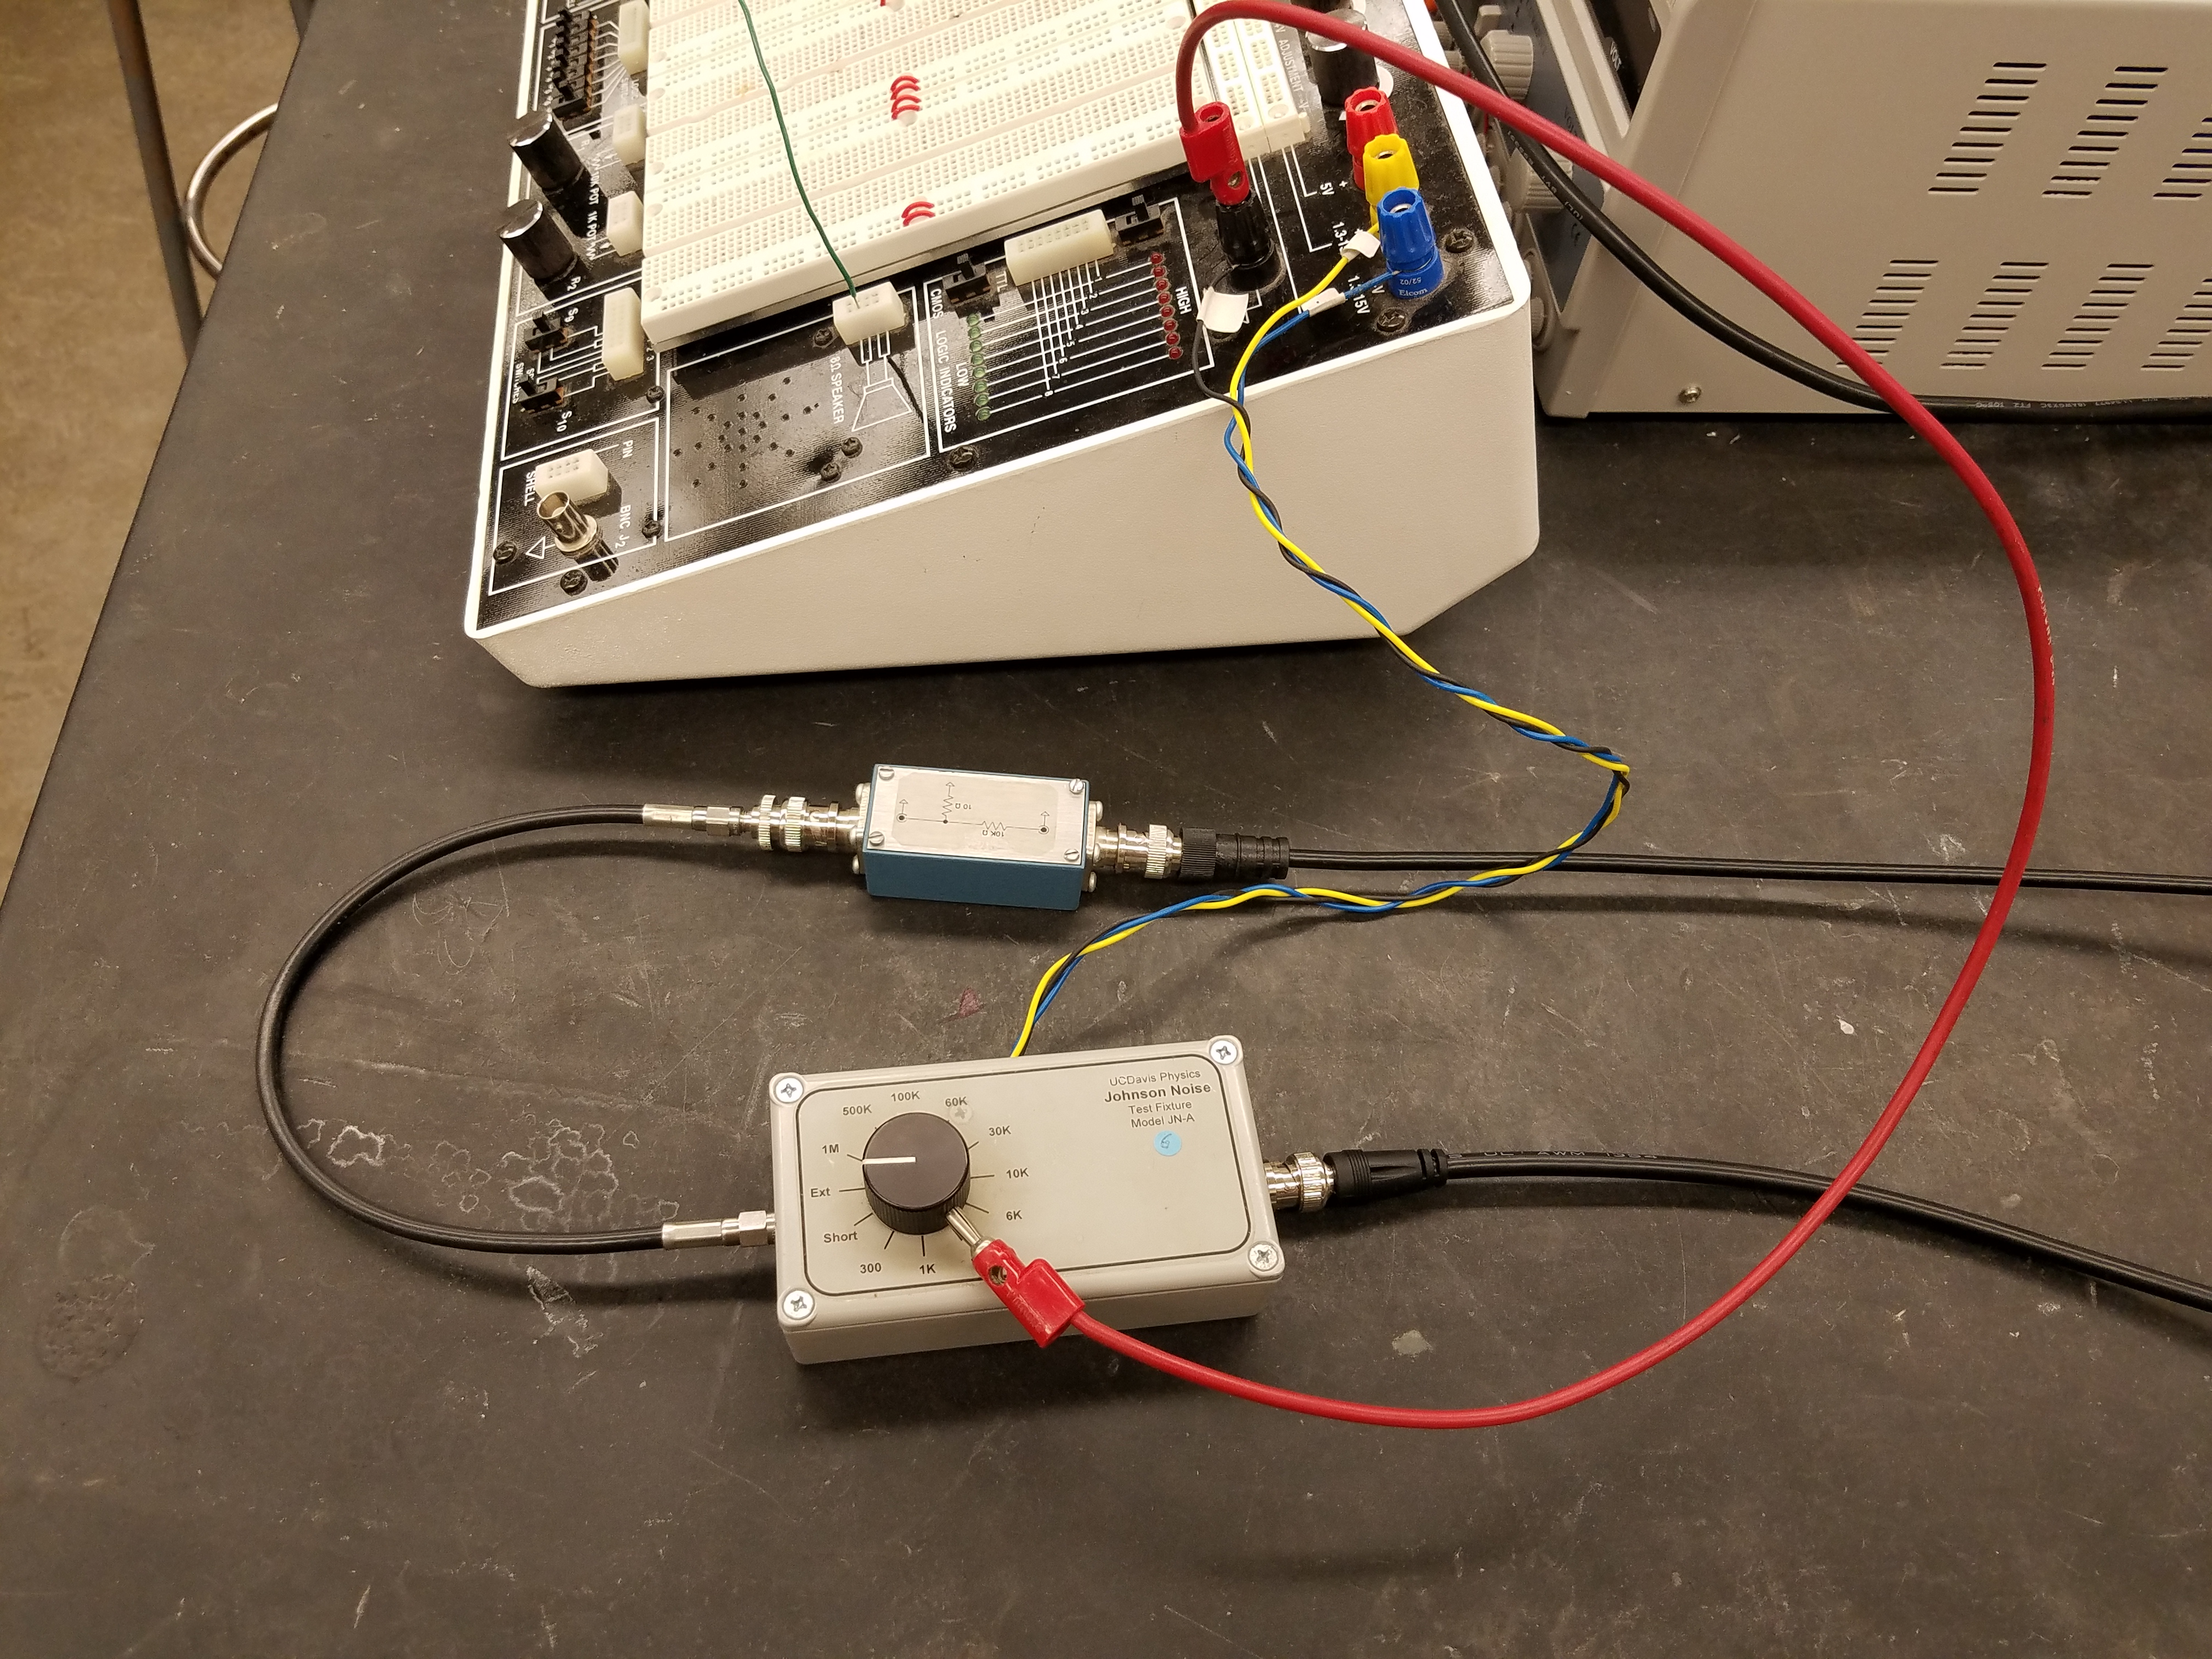
\includegraphics[width=0.65\textwidth]{figs/jn_setup.jpg}}
\end{center}
\caption{\label{fig:plan} Connections to the Johnson Noise device.  Note the banana plug used to reduce noise from the knob acting as an antenna!}
\end{figure}

In this section, we will measure the gain of the Johnson Noise device as function of frequency.

Obtain a Johnson Noise (JN) measurement device (Model JN-A or JN-B) and note the serial number (e.g. \#4).  These are high gain devices that are very susceptible to damage.  Do not drive them directly from a function generator, but use a 1000:1 attenuated, taking care that the small resistor is toward the JN device (else you will reduce voltage by a factor 999/1000, and likely damage the equipment!)  

The JN devices are very sensitive, easily pickup noise, and ring at a characteristic frequency of about $27~{\rm kHz}$.  The tuning knob in particular picks up noise.  An old version banana plug cable plugged into the knob at the set screw grounds the knob, eliminated this source of noise.  The effect can be quite dramatic. 

Adjust the supply levels on your bench-top supply to $+12~{\rm V}$ and $-12~{\rm V}$.  Then, with the supply turned off, connect the JN device to power and ground, as labeled on the wires.  Once connected, power the device on and adjust the current thresholds to just slightly above where the supplies become current limited.  Under normal operation, the JN device should draw about $20~\rm mA$ from each supply... keep an eye on it.  If one of the supplies is inadvertently disconnected, the circuit latches in a high current state, which should be avoided if possible.

Set your function generator to produce a sine wave with $V_{\rm rms} = 100~\rm mV$ and $f = 1~\rm kHz$.  Connect the function generator to channel 1 of your scope, then to the $1000:1$ attenuator, and then to your JN device,  The output of the JN device should then be plugged directly into the scope channel 2.

\begin{figure}[htbp]
\begin{center}
{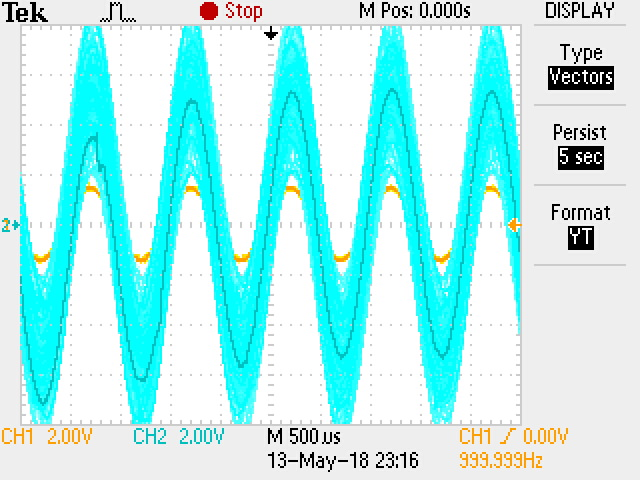
\includegraphics[width=0.65\textwidth]{figs/gaintrouble.jpg}}
\end{center}
\caption{\label{fig:gaintrouble} The output of the Johnson Noise device bounces around a lot due to low frequency noise.  Here the output is shown with display persistance.}
\end{figure}

Make a series of gain measurements at different frequencies that will allow to determine the integral
\begin{displaymath}
\int_{-\infty}^{\infty} df g(f)^2.
\end{displaymath}
While making the gain measurement, you will see that the output of the Johnson Noise seems to bounce around.  The effect can be seen if Fig.~\ref{fig:gaintrouble}.  There is a significant amount of low frequency noise in the output.  I found the best approach was to trigger on the AC line, which allows you to find a region of the plot with relatively little 60 Hz noise.  Use the scopes Measure capability to find the RMS voltage of the input and output of the Johnson Noise.  This is likely the major systematic uncertainty in your measurement, so spend some time thinking about how to quantify it. 

You might be tempted to try and use your DMM to measure the RMS voltage of your signal, but this is a mistake.  Your DMM is designed to measure 60~\rm Hz AC.

\section{Johnson Noise Measurement}

Turn down the function generator and disconnect it from the JN device.

Turn the knob to select a resistor, and note the RMS voltage from the scope.  Repeat this measurement for every resistance.  

These measurements, plus the gain measurement, should allow you to calculate $\kb$.

\section{Arduino Voltage Interface}

The Arduino analog inputs have an input voltage range from 0 to 5 V, but our signals after amplification can reach the supply levels as $\pm12~{\rm V}$.  We'll need an interface circuit to provide these signals at a voltage level appropriate for the Arduino.  

\begin{figure}[htbp]
\begin{center}
%\begin{overpic}[width=0.5\textwidth,grid,tics=10]{adder.pdf}
\begin{overpic}[width=0.5\textwidth]{figs/adder.pdf}  
 \put (23,52) {$R_1$}
 \put (23,41) {$R_2$}
 \put (23,24) {$R_3$}
 \put (63,24) {$R_4$}
 \put (60,45) {LM324}
 \put (6,47) {$V_{\rm in}$}
 \put (6,34) {$V_{\rm ref}$}
 \put (82,35) {$V_{\rm out}$}
\end{overpic}
%{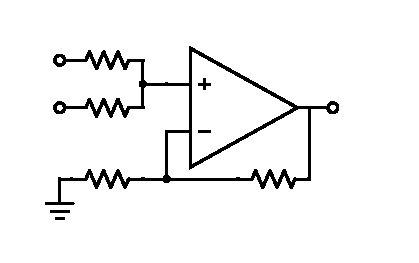
\includegraphics[width=0.65\textwidth]{adder.pdf}}
\end{center}
\caption{\label{fig:offset} A DC level-shifter with unit gain.}
\end{figure}

An appropriate circuit is shown in Fig.~\ref{fig:offset}, where you can use $R_1=R_4=15~{\rm k\Omega}$, 
$R_2=R_3=30~{\rm k\Omega}$. 
 

\section{Gain Determination}

For calibration, note that the peak of periodogram resulting from a sine wave with amplitude A will be:
\begin{displaymath}
\frac{T}{2}|A|^2
\end{displaymath}

\section{Power Spectrum Analysis}

\end{document}


